\documentclass[border=1pt]{standalone}
% ---------------------------------------------------------------------------
% Shared style for the MOSAIC / CRYSTAL TOMM figures.
% Compile each fig_*.tex with LuaLaTeX (standalone). Sized for acmart
% "acmsmall" (TOMM): \textwidth = 13.9 cm, so every figure is drawn at
% final size and is included with width=\textwidth (no rescaling of text).
% Fonts: Libertinus Sans + Inconsolata (acmart uses Libertine + Inconsolata).
% ---------------------------------------------------------------------------
\usepackage{fontspec}
\setmainfont{LibertinusSans}[Path=fonts/, Extension=.otf,
  UprightFont=*-Regular, BoldFont=*-Bold, ItalicFont=*-Italic]
\setmonofont{Inconsolata}[Path=fonts/, Extension=.otf,
  UprightFont=*-Regular, BoldFont=*-Bold, Scale=0.98]
\usepackage{unicode-math}
\setmathfont{LibertinusMath-Regular.otf}[Path=fonts/]

\usepackage{tikz}
\usetikzlibrary{positioning,fit,calc,arrows.meta,backgrounds,
  shapes.misc,shapes.geometric,decorations.pathreplacing,patterns.meta}

% Okabe-Ito palette (colour-blind safe) + tints -------------------------------
\definecolor{oiBlue}{HTML}{0072B2}
\definecolor{oiOrange}{HTML}{E69F00}
\definecolor{oiSky}{HTML}{56B4E9}
\definecolor{oiGreen}{HTML}{009E73}
\definecolor{oiVerm}{HTML}{D55E00}
\definecolor{oiPurple}{HTML}{CC79A7}
\definecolor{oiYellow}{HTML}{F0E442}
\definecolor{ink}{HTML}{1A1A1A}
\definecolor{muted}{HTML}{5C5C5C}
\definecolor{rule}{HTML}{9A9A9A}

\definecolor{oursFill}{HTML}{DDEBF7}
\definecolor{oursDraw}{HTML}{0072B2}
\definecolor{modFill}{HTML}{FCEFD2}
\definecolor{modDraw}{HTML}{B57600}
\definecolor{upFill}{HTML}{F1F1F1}
\definecolor{upDraw}{HTML}{7D7D7D}
\definecolor{failFill}{HTML}{FBE3D6}
\definecolor{okFill}{HTML}{D9F0E8}

% Sequence colours (as in the packetization study)
\definecolor{seqSOL}{HTML}{0072B2}
\definecolor{seqTHA}{HTML}{009E73}
\definecolor{seqLON}{HTML}{CC79A7}

% Typography -----------------------------------------------------------------
\newcommand{\figfont}{\fontsize{7.5}{9}\selectfont}
\newcommand{\smallfig}{\fontsize{6.5}{7.8}\selectfont}
\newcommand{\tinyfig}{\fontsize{6}{7.2}\selectfont}
\newcommand{\code}[1]{{\ttfamily #1}}

% Provenance encoding: colour AND line style (grayscale safe) ------------------
%  ours      = new component written by us      (blue, solid 0.9 pt)
%  modified  = upstream component we patched    (orange, dashed 0.8 pt)
%  upstream  = used unmodified / third party    (grey, solid 0.45 pt)
\tikzset{
  base/.style={rectangle, rounded corners=1.6pt, align=center,
    inner xsep=3pt, inner ysep=2.6pt, font=\figfont, text=ink,
    execute at begin node={\hyphenpenalty=10000\exhyphenpenalty=10000}},
  ours/.style={base, fill=oursFill, draw=oursDraw, line width=0.9pt},
  mod/.style={base, fill=modFill, draw=modDraw, line width=0.8pt,
    dash pattern=on 2.6pt off 1.4pt},
  up/.style={base, fill=upFill, draw=upDraw, line width=0.45pt},
  dead/.style={base, fill=white, draw=oiVerm, line width=0.6pt,
    dash pattern=on 1.2pt off 1.2pt, text=oiVerm},
  note/.style={font=\smallfig, text=muted, align=left,
    execute at begin node={\hyphenpenalty=10000\exhyphenpenalty=10000}},
  lab/.style={font=\smallfig\itshape, text=muted},
  zone/.style={draw=rule, line width=0.45pt, rounded corners=3pt,
    dash pattern=on 0.6pt off 1.1pt},
  zonetitle/.style={font=\figfont\bfseries, text=ink, anchor=west,
    inner xsep=2pt, inner ysep=1pt, fill=white, xshift=2.5mm},
  flow/.style={-{Stealth[length=4pt,width=3.2pt]}, line width=0.65pt,
    draw=ink},
  dflow/.style={flow, dash pattern=on 2pt off 1.4pt},
  ctrl/.style={-{Stealth[length=3.4pt,width=2.8pt]}, line width=0.5pt,
    draw=muted},
  failflow/.style={-{Stealth[length=4pt,width=3.2pt]}, line width=0.6pt,
    draw=oiVerm, dash pattern=on 1.4pt off 1.2pt},
  stepc/.style={circle, fill=ink, text=white, inner sep=0pt,
    minimum size=8.5pt, font=\tinyfig\bfseries},
  tag/.style={font=\tinyfig\bfseries, inner sep=1pt},
}

% Legend for the provenance encoding -------------------------------------------
\newcommand{\provlegend}[1]{% #1 = anchor coordinate (north west)
  \begin{scope}[shift={(#1)}]
    \node[ours, minimum width=6mm, minimum height=2.6mm, inner sep=0pt]
      (lg1) at (0,0) {};
    \node[anchor=west, font=\smallfig] at (lg1.east) {new (this work)};
    \node[mod, minimum width=6mm, minimum height=2.6mm, inner sep=0pt]
      (lg2) at (2.6,0) {};
    \node[anchor=west, font=\smallfig] at (lg2.east) {upstream, patched by us};
    \node[up, minimum width=6mm, minimum height=2.6mm, inner sep=0pt]
      (lg3) at (6.2,0) {};
    \node[anchor=west, font=\smallfig] at (lg3.east) {upstream / third party, unmodified};
  \end{scope}}

\newcommand{\bx}[2]{{\bfseries #1\par}\vspace{0.6pt}{\smallfig #2\par}}
\begin{document}
\figfont
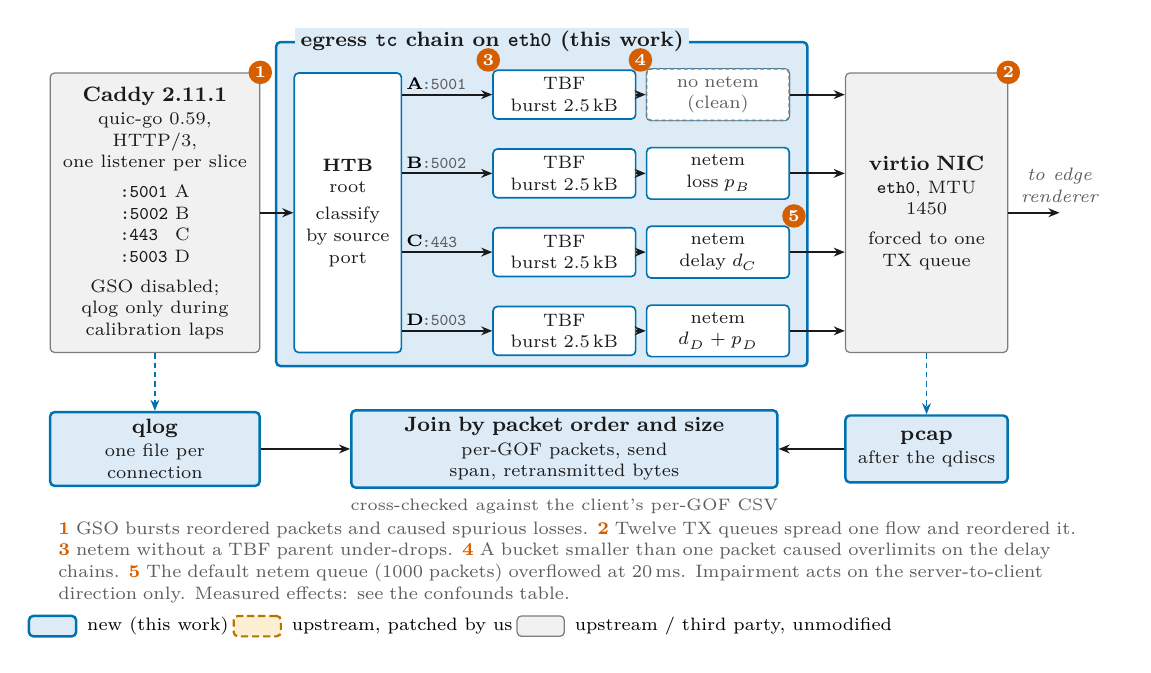
\begin{tikzpicture}[x=1cm,y=1cm]
  \tikzset{q/.style={base, fill=white, draw=oursDraw, line width=0.6pt, font=\smallfig,
              text width=1.6cm, minimum height=0.62cm},
           cls/.style={font=\smallfig, anchor=east, align=right},
           badge/.style={stepc, fill=oiVerm}}

  % ---------------------------- Caddy ------------------------------------------
  \node[up, text width=2.45cm, minimum height=3.55cm] (cad) at (1.4,3.05)
    {\bx{Caddy 2.11.1}{quic-go 0.59, HTTP/3,\\one listener per slice\\[3pt]
      \code{:5001} A\\\code{:5002} B\\\code{:443}\phantom{0} C\\\code{:5003} D\\[3pt]
      GSO disabled;\\qlog only during\\calibration laps}};
  \node[badge] at (cad.north east) {1};

  % ---------------------------- qdisc tree --------------------------------------
  \node[q, text width=1.15cm, minimum height=3.55cm] (htb) at (3.85,3.05) {\textbf{HTB}\\root\\[2pt]classify\\by source\\port};
  \foreach \n/\y/\l/\ne in {A/4.55/:5001/{no netem\\(clean)},
                           B/3.55/:5002/{netem\\loss $p_B$},
                           C/2.55/:443/{netem\\delay $d_C$},
                           D/1.55/:5003/{netem\\$d_D$ + $p_D$}}{
    \node[font=\tinyfig\bfseries, anchor=south west, inner sep=1pt] (L\n) at (4.55,\y+0.02) {\n};
    \node[font=\tinyfig\ttfamily, text=muted, anchor=south west, inner sep=1pt] at (4.75,\y+0.02) {\l};
    \node[q] (T\n) at (6.6,\y) {TBF\\burst 2.5\,kB};
    \node[q] (N\n) at (8.55,\y) {\ne};
    \draw[flow] (htb.east |- T\n.west) -- (T\n.west);
    \draw[flow] (T\n) -- (N\n);
  }
  \node[q, draw=upDraw, fill=white, dash pattern=on 1.5pt off 1pt, text=muted] at (NA) {no netem\\(clean)};
  \begin{scope}[on background layer]
    \node[ours, fit=(htb)(TA)(NA)(TD)(ND)(LA), inner sep=2.2mm, yshift=1.1mm, fill=oursFill] (zq) {};
  \end{scope}
  \node[zonetitle, fill=oursFill] at (zq.north west) {egress \code{tc} chain on \code{eth0} (this work)};
  \node[badge] at ($(TA.north west)+(-0.05,0.12)$) {3};
  \node[badge] at ($(TA.north east)+(0.05,0.12)$) {4};
  \node[badge] at ($(NC.north east)+(0.05,0.12)$) {5};
  \draw[flow] (cad.east |- htb.west) -- (htb.west);

  % ---------------------------- NIC + link -------------------------------------
  \node[up, text width=1.85cm, minimum height=3.55cm] (nic) at (11.2,3.05)
    {\bx{virtio NIC}{\code{eth0}, MTU 1450\\[3pt]forced to one\\TX queue}};
  \node[badge] at (nic.north east) {2};
  \foreach \n in {A,B,C,D}{ \draw[flow] (N\n.east) -- (nic.west |- N\n.east); }
  \draw[flow] (nic.east) -- ++(0.65,0) node[above, lab, align=center, anchor=south] {to edge\\renderer};

  % ---------------------------- measurement plane -------------------------------
  \node[ours, text width=2.45cm, minimum height=0.85cm] (ql) at (1.4,0.05)
    {\bx{qlog}{one file per connection}};
  \node[ours, text width=1.85cm, minimum height=0.85cm] (pc) at (11.2,0.05)
    {\bx{pcap}{after the qdiscs}};
  \node[ours, text width=5.2cm, minimum height=0.85cm] (jn) at (6.6,0.05)
    {\bx{Join by packet order and size}{per-GOF packets, send span, retransmitted bytes}};
  \draw[dflow, draw=oiBlue] (cad.south) -- (ql.north);
  \draw[dflow, draw=oiBlue] (nic.south) -- (pc.north);
  \draw[flow] (ql) -- (jn);
  \draw[flow] (pc) -- (jn);
  \node[font=\tinyfig, text=muted, anchor=north] at (jn.south) {cross-checked against the client's per-GOF CSV};

  % ---------------------------- confound key ------------------------------------
  \node[note, anchor=north west, text width=13.4cm] at (0.05,-0.75)
    {\textcolor{oiVerm}{\textbf{1}}~GSO bursts reordered packets and caused spurious losses.
     \textcolor{oiVerm}{\textbf{2}}~Twelve TX queues spread one flow and reordered it.
     \textcolor{oiVerm}{\textbf{3}}~netem without a TBF parent under-drops.
     \textcolor{oiVerm}{\textbf{4}}~A bucket smaller than one packet caused overlimits on the delay chains.
     \textcolor{oiVerm}{\textbf{5}}~The default netem queue (1000 packets) overflowed at 20\,ms. Impairment acts on the server-to-client direction only. Measured effects: see the confounds table.};

  \provlegend{0.1,-2.2}
\end{tikzpicture}
\end{document}
